\chapter{Setup and Implementation}
\label{chap:3}
%
This chapter is focused on the implementation of the probabilistic intention prediction algorithm. \\
The algorithm was written in Python and C++ programming languages and tested, \gls{ROS}. As mentioned in Chapter 1, \gls{ROS} is a framework where testing cases can be easily developed and tested. In current visualization framework, we tested $2$ environments consisting of a static map for T and X intersections and the car itself (model is created with two cars which can be simulated simultaneously, but for proving the concept we decided to work with only one car at the time). \\
In order to visualize simulation \gls{RViz}, which is a 3D visualizer for showing data and state information from \gls{ROS}, was used. A snapshot of the simulation environment is in Figure~\ref{fig:ROS1}. 

\begin{figure}[H]
	\centering  	
	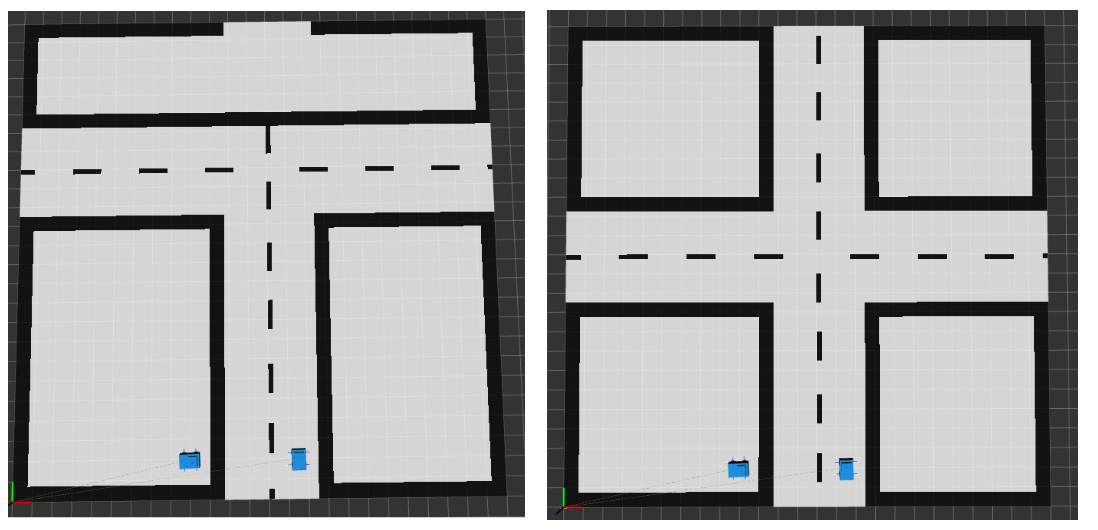
\includegraphics[width=10cm]{img/RosMaps.png}
	\caption{Experiments were made having two environments: T and X intersection. The figure illustrates how these  environments look like in \gls{RViz} - \gls{ROS} visualization tool, where simulations were run}
	\label{fig:ROS1}    
\end{figure}

As mentioned in Chapter 3, this project has several testing cases. Methods tested with having two types of trajectories. The first one was pre-recorded trajectories and the second one was real time trajectories. Data from every run is stored in order to analyze and deduce what effect each method has on algorithm performance. Parameters and results for the run are independent and tested several times in a specific environment to be able to draw conclusions from the results we received during the testing phase.

\section{Data Collection}

Collecting data was one of the first steps for implementing a probabilistic intention prediction algorithm because, in order to recognize and predict intentions, common features for each movement classes need to be described (algorithm has to learn the features from recorded demonstrations in training process). We did not use any existing \glspl{DB} - we created \glspl{DB} for trajectories of interests by ourselves.  \\
At the beginning, we collected data only from \gls{ROS} simulations and later one we collected data from a real car.

\subsection{Data Collection with \gls{ROS}}

To be able to control car in \gls{ROS} and its visualization in \gls{RViz} environment, \gls{ROS} joy package was used. This package allows us to connect a physical joystick to \gls{ROS} and provides all necessary drivers and libraries. To be able to record and store data which we collected by making experiments Python GUI application was used. On the left of Figure~\ref{fig:GUIandJOY} brief scheme of data collection is shown and on the right side GUI application window is illustrated.

\begin{figure}[H]
	\centering  	
	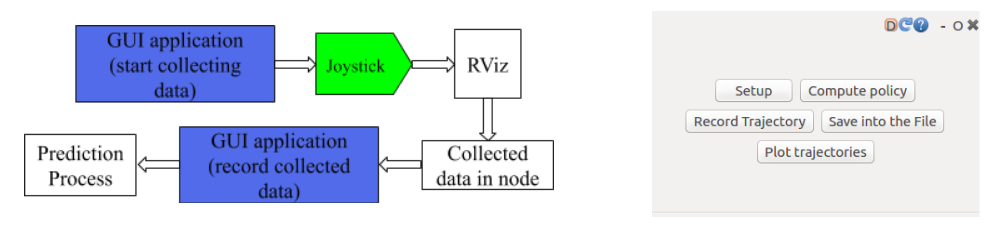
\includegraphics[width=17cm]{img/ROS+GUI.png}
	\caption{On the right side graphical user interface is shown, it helps with the simulated data recording process, left side briefly illustrates data collection process, using \gls{ROS} Joystick node}
	\label{fig:GUIandJOY}    
\end{figure}

Joy package is a \gls{ROS} driver for a "generic Linux joystick".The package consists of joy\_node, a node which allows communication between a generic joystick and \gls{ROS}. Joy message, which contains information about the current state of each button on joystick is published by node \cite{ROSjoy}, having this information command start to move, turn to any direction, stop is sent to the object we want to control in \gls{ROS} environment.  \\
When all necessary systems were connected together and ready to be used we pressed the button "Record Trajectory" in GUI application and give a start command to a car, by controlling joystick, while the car is moving with a help of joystick position of the car is stored every few milliseconds.  When "car's journey" is done and we want to store recorded and stored data to a file we again pressed the button "Save into the File" in GUI application and one trajectory is recorded. This process needed to be repeated every time when we want to record trajectory.\\
As mentioned above there are two map types: X and T intersections.  For X-intersection a various number of trajectories for movement to the right, straight and left were recorded, while for T-intersection only movement t the right and left was recorded.

\subsection{Data Collection from Real Car}

TU-Darmstadt has autonomous driving working group aDDa, which is developing software and hardware to make a real autonomous car (Figure~\ref{fig:ReadCAr}). We made test drives to collect data from a real car and ran our probabilistic intention prediction algorithm on this dataset. 

\begin{figure}[H]
	\centering  	
	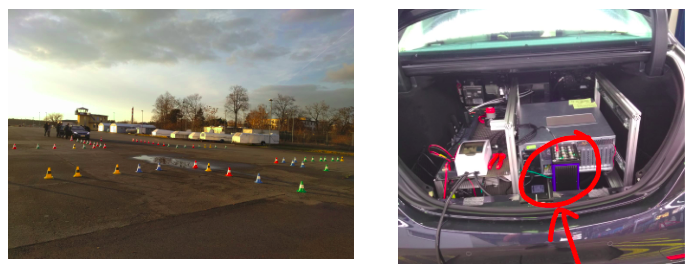
\includegraphics[width=17cm]{img/realCar.png}
	\caption{On the left side is the picture shows how data collection looked like and the right side shows where \gls{ADMA} sensor is in the car}
	\label{fig:ReadCAr}    
\end{figure}

We were interested in only \gls{ADMA} data (\gls{ADMA} - the high-precision gyro measuring system specially developed for vehicle dynamics measurements), which we recorded using \gls{ROS} recording node while the car was moving. Figure~\ref{fig:ReadCAr} includes a picture of the test drive environment and \gls{ADMA} position in the car. After recording data, we had a *.bag file with all information we can get from \gls{ADMA}: acceleration, speed and position of moving vehicles in three-dimensional (x, y, z) axes. For our working purposes, we were only interested in position data, due to that the listener node, listening the only position was written (we run listener \gls{ROS} node on *.bag information file from \gls{ADMA} and we save all recorded positions to the *.csv file). \\
Real Car data, recorded with \gls{ADMA} did not have the same start position (and not even close ones). Since this gave some inaccuracy for our algorithm, we converted data to a Cartesian coordinate system, with the starting point ($14.5$, $2.0$) and then when a new position arrives, we computed the difference of the new position to the first real position (e.g. first three points for one trajectory after this changes look like this: [[$14.5$, $2.0$], [$14.7$, $2.4$], [$14.9$, $2.8$], ....] \\
After these changes, we have a set of reasonably represented data from the real car.

\section{Brief Algorithm Explanation}

Following Chapter 3, the whole framework starts to work with map recognition, when the type of the map is known, initial belief ($b_{0}$) is calculated. When recognized map is X intersection initial belief is ($b_{0}\text{[right, straight, left]} = (0.333, 0.333, 0.333)$), when we are working with T intersection, initial belief is $b_0 \text{[left, right]}= (0.533, 0.467)$. Map recognition is introduced in Chapter 3, Section 3.1.
Once we know the map type we are preparing our demonstrations for learning initial probabilistic prediction model. Unification of all demonstrations in our \gls{DB} is made using interpolation, detailed explanation is in Chapter 3, Section 3.2. After interpolation is done our algorithm is learning initial probabilistic model: in X intersection we are working with $3$, while in T intersection with $2$ movement classes. How algorithm is learning initial probabilistic prediction model is described in Chapter 3, Section 3.4.
Section 3.4 in Chapter 3, explains how belief is calculated and updated. Prediction is making until trajectory is over, due to that after every step algorithm is checking if movement still happening, if yes, the last belief is updated and new prediction is made, while trajectory ends. If current time step is the last for trajectory then algorithm stops. The brief scheme of algorithm workflow is in Figure~\ref{fig:flow}

\begin{figure}[H]
	\centering  	
	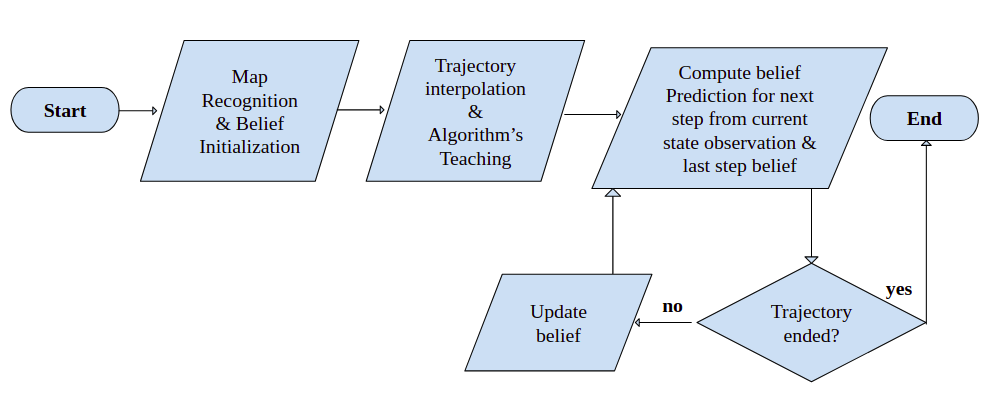
\includegraphics[width=13cm]{img/flow.png}
	\caption{The workflow of the probabilistic intention prediction algorithm. Starting with the map recognition process, according to the map initial belief is initialized. After that trajectories, unification and initial prediction model creation happened. The last step when we have all this initial information is to make predictions for that we need last belief, current car position and learned data, when prediction is made, it is checking if trajectory is over, if yes, then algorithm is ending, if not, then cycle with updated belief and new observation is continuing}
	\label{fig:flow}    
\end{figure}

As an additional part of thesis trajectory scaling process was introduced and checked. Scaling was introduced following the common logic that making more belief updates, i.e. having more time steps in trajectory, would allow to have better precision. The problem with more time steps is the longer computation time, which in critical infrastructures, as vehicles, should be as small as possible. We wanted to achieve precision of $100$ time steps, but having only $10$ steps in trajectory. \\
On more additional part of thesis, when we managed to predict step by step movement, we wanted to see if we can predict all future trajectory. We tested that, using \gls{ProMPs} and approach, proposed in \cite{ProMPs}. \\
The results for this and other methods, described in this chapter can be found in flowing Chapter~\ref{chap:4} \textbf{"Experiments and Results"}.




